\section{Численный метод}
\subsection{Численный метод в одномерном случае}
Как следует из \ref{model-1d}, для моделирования сплошной среды можно использовать уравнения в эйлеровой, лагранжевой или смешанной форме. При этом рассчётная сетка может быть неподвижной или двигаться вместе с частицами тела. Возможны также промежуточные варианты, когда сетка движется вместе с телом, но не "вморожена" в него, для большего постоянства расстояния между рассчётными узлами.

Из наиболее простых и распространённых вариантов следует отметить следующие два:
\begin{itemize}
\item Неподвижная сетка и эйлеровы уравнения. К его недостаткам можно отнести сложность реализации при макросокопических деформациях тел.
\item "Вмороженная" в тело сетка и уравнения в смешанной форме, где дифференцирование по времени подразумевается в фиксированной частице тела, а пространственная производная рассчитывается именно из координат рассчётных узлов в неподвижном пространстве.
\end{itemize}
В любом случае все указанные методы моделируют одну и ту же физическую систему и должны давать одинаковые результаты в пределах их точности и применимости. 

В данной работе был реализован второй метод. Он подразумевает расщепление шага по времени на два физических процесса: распространение возмущения в веществе и перенос самого вещества. 

Расчёт распространения возмущения осуществляется методом, являющимся упрощением его трёхмерного аналога, описанного в \ref{hyperbolic}. Сама по себе реализация движения узлов сетки со вторым порядком точности по времени также не вызывает затруднений.

В методе первого порядка достаточно в конце (или в начале, что несущественно) каждого расчёта распространения возмущения в веществе перемещать узел сетки на расстояние $x_{n+1} - x_{n} = v_{n+1}\tau$ или $v_{n}\tau$. Схема данного простейшего расщепления показана на рис.\ref{pic:splitting}, a.

Однако для того, чтобы расчёт целиком проходил со вторым порядком точности по времени, необходимо осуществить более симметричное расщепление, чем вышеописанное. Его схема показана на рис.\ref{pic:splitting}, b. На очередном шаге сначала за половинное время $\tau/2$ со вторым порядком точности перемещаются рассчётные узлы. Для этого приходится рассчитать скорости в узлах в момент $t_n + \tau/2.$ После этого производится расчёт скоростей и напряжений на новом слое $t_{n+1}$. При этом для аппроксимации берутся значения скоростей и напряжений в $t_n,$ а координаты узлов -- только что пересчитанные. После этого окончательно сдвигается сетка.

\begin{figure}[h!]
\begin{minipage}{0.47\linewidth}
\center{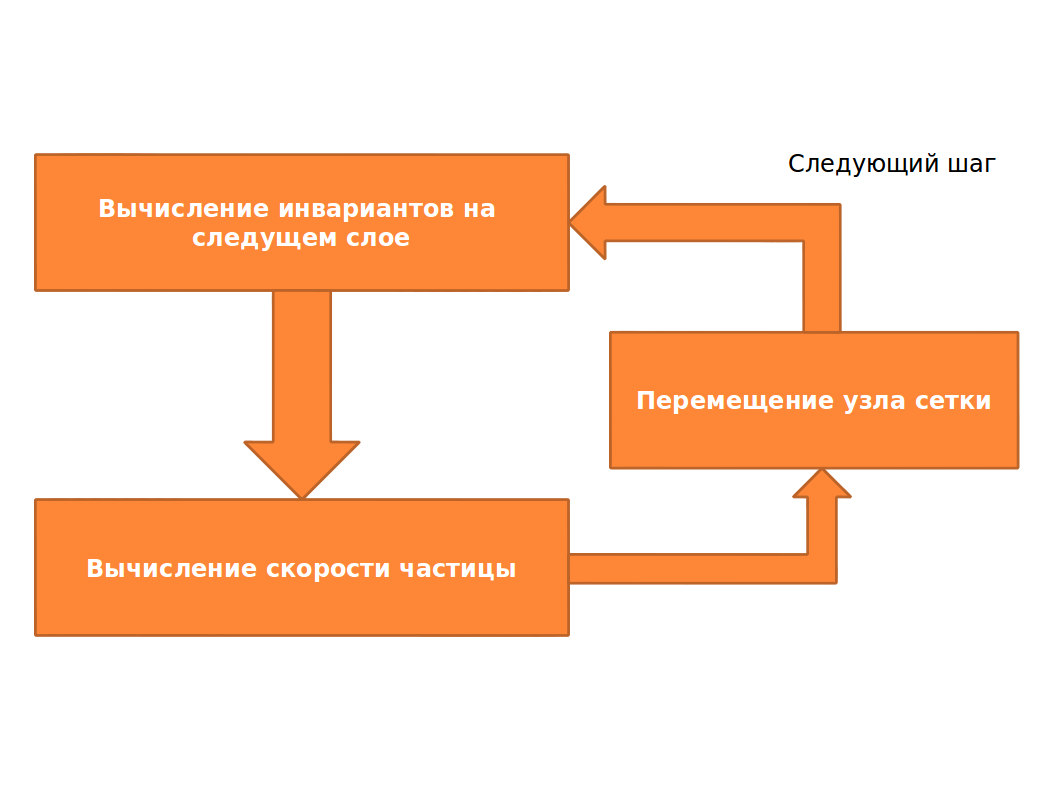
\includegraphics[width=1\linewidth]{png/1d/first-order.png}} a)
\end{minipage}
\begin{minipage}{0.47\linewidth}
\center{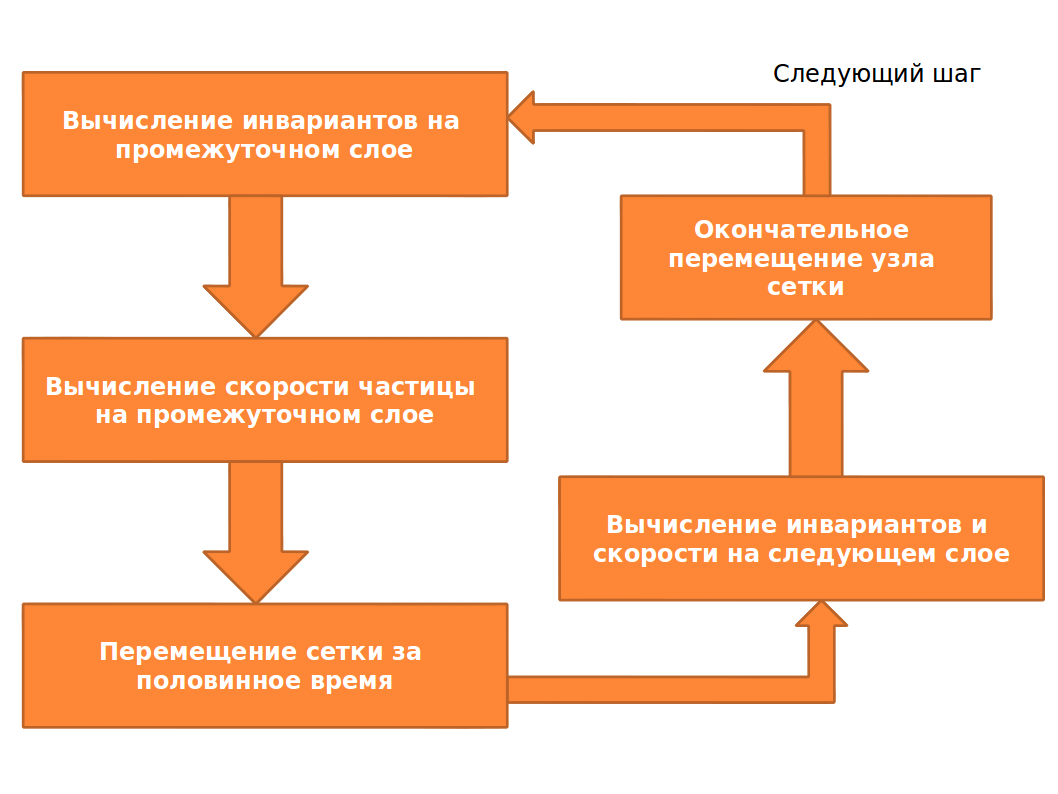
\includegraphics[width=1\linewidth]{png/1d/second-order.png}} b)
\end{minipage}
\caption{Схема расщепления на процессы распространения возмущения в веществе и переноса частиц вещества a) певого, b) второго порядка точности.}
\label{pic:splitting}
\end{figure} 

Далее рассмотрим идеи численного метода в трёхмерной постановке.
\subsection{Расщепление на упругую и пластическую части}
Пластическая задача решается расщеплением на два физических процесса: упругая деформация и пластическое течение. Расщепление проводилось на каждом из трёх подшагов по пространственным координатам, которые будут описаны ниже. На этапе предиктора расчёт значений на новом временном слое делается как для линейно-упругого тела. Затем, в случае выхода напряжений за пределы поверхности текучести, пластический корректор возвращает их обратно на $f(\sigma_{ij})=0$.
\subsection{Решение линейно-упругой части задачи}
\subsubsection{Матричная форма уравнений линейной упругости}
Уравнения \ref{rheology_equations} и \ref{tensor_qijkl} можно переписать в матричной
форме:
\begin{equation}
\label{matrix_equation}
\frac{\partial}{\partial{t}}\vec{u}+\mathbf{A}_x\frac{\partial}{\partial{x}}\vec{u}+
\mathbf{A}_y\frac{\partial}{\partial{y}}\vec{u}+
\mathbf{A}_z\frac{\partial}{\partial{z}}\vec{u}=\vec{f}.
\end{equation}
Здесь
$\vec{u}=\{v_x,v_y,v_z,\sigma_{xx},\sigma_{xy},\sigma_{xz},\sigma_{yy},\sigma_{yz},\sigma_{zz}\}^T$
-- вектор искомых функций, $\vec{f}$ -- вектор правых частей той же размерности,
$x,y,z$ --  независимые пространственные переменные, $t$ -- время,
\begin{displaymath}
\mathbf{A}_x =
\left( \begin{array}{cccccccccccc}
0 & 0 & 0 & -\frac 1 \rho & 0 & 0 & 0 & 0 & 0 \\ 
0 & 0 & 0 & 0 & -\frac 1 \rho & 0 & 0 & 0 & 0 \\ 
0 & 0 & 0 & 0 & 0 & -\frac 1 \rho & 0 & 0 & 0 \\ 
-\lambda-2\mu & 0 & 0 & 0 & 0 & 0 & 0 & 0 & 0 \\ 
0 & -\mu & 0 & 0 & 0 & 0 & 0 & 0 & 0 \\ 
0 & 0 & -\mu & 0 & 0 & 0 & 0 & 0 & 0 \\ 
-\lambda & 0 & 0 & 0 & 0 & 0 & 0 & 0 & 0 \\ 
0 & 0 & 0 & 0 & 0 & 0 & 0 & 0 & 0 \\ 
-\lambda & 0 & 0 & 0 & 0 & 0 & 0 & 0 & 0  
\end{array} \right),
\end{displaymath} 
\begin{displaymath}
\mathbf{A}_y =
\left( \begin{array}{cccccccccccc}
0 & 0 & 0 & 0 & -\frac 1 \rho & 0 & 0 & 0 & 0 \\ 
0 & 0 & 0 & 0 & 0 & 0 & -\frac 1 \rho & 0 & 0 \\ 
0 & 0 & 0 & 0 & 0 & 0 & 0 & -\frac 1 \rho & 0 \\ 
0 & -\lambda & 0 & 0 & 0 & 0 & 0 & 0 & 0 \\ 
-\mu & 0 & 0 & 0 & 0 & 0 & 0 & 0 & 0 \\ 
0 & 0 & 0 & 0 & 0 & 0 & 0 & 0 & 0 \\ 
0 & -\lambda-2\mu & 0 & 0 & 0 & 0 & 0 & 0 & 0 \\ 
0 & 0 & -\mu & 0 & 0 & 0 & 0 & 0 & 0 \\ 
0 & -\lambda & 0 & 0 & 0 & 0 & 0 & 0 & 0  
\end{array} \right),
\end{displaymath}
\begin{displaymath}
\mathbf{A}_z =
\left( \begin{array}{cccccccccccc}
0 & 0 & 0 & 0 & 0 & -\frac 1 \rho & 0 & 0 & 0 \\
0 & 0 & 0 & 0 & 0 & 0 & 0 & -\frac 1 \rho & 0 \\
0 & 0 & 0 & 0 & 0 & 0 & 0 & 0 & -\frac 1 \rho \\
0 & 0 & -\lambda & 0 & 0 & 0 & 0 & 0 & 0 \\
0 & 0 & 0 & 0 & 0 & 0 & 0 & 0 & 0 \\
-\mu & 0 & 0 & 0 & 0 & 0 & 0 & 0 & 0 \\
0 & 0 & -\lambda & 0 & 0 & 0 & 0 & 0 & 0 \\
0 & -\mu & 0 & 0 & 0 & 0 & 0 & 0 & 0 \\
0 & 0 & -(\lambda+2\mu) & 0 & 0 & 0 & 0 & 0 & 0
\end{array} \right).
\end{displaymath}
\subsubsection{Гиперболические свойства систем уравнений линейной упругости}
\label{hyperbolic}
Рассмотрим сначала одномерное уравнение вида
\begin{equation}
\frac{\partial}{\partial{t}}\vec{u}+\mathbf{A}\frac{\partial}{\partial{x}}\vec{u}=\vec{f}.
\label{advection_equation}
\end{equation}
Если матрица $\mathbf{A}$ имеет полный набор вещественных собственных значений, 
то такое уравнение называется гиперболическим, и его решения соответствуют 
процессам, которые носят волновой характер. В этом случае справедливо разложение:
$$\mathbf{A}=\mathbf\Omega^{-1}\mathbf\Lambda\mathbf\Omega,$$
где $\mathbf\Omega$ -- матрица, составленная из векторов ${\vec\omega_i}$, где
$\vec\omega_i$ есть собственные векторы матрицы $\mathbf A$,
удовлетворяющие соотношениям
$$\vec\omega_i\mathbf A=\lambda_i\vec\omega_i,$$
а $\mathbf\Lambda=diag\{\lambda_i\}$ -- диагональная матрица собственных
значений.
В предположении независимости компонент матрицы $\mathbf{A}$ от времени и координаты, домножив уравнение \ref{advection_equation} слева на $\Omega$, получаем
уравнение
$$\frac{\partial}{\partial t}\Omega{\vec u}+
\Lambda\frac{\partial}{\partial x}\Omega{\vec u}=\Omega{\vec f},$$
которое после перехода к Римановым инвариантам ${\vec v}=\Omega{\vec u}$
распадается на $n$ одномерных уравнений вида
\begin{equation}
\frac{\partial}{\partial t}{v_i}+\lambda_i\frac{\partial}{\partial
x}{v_i}={{\tilde f}_i},
\label{advection_equation_splitted}
\end{equation}
где ${{\tilde f}_i}=(\Omega{\vec f})_i$.
Таким образом, решение уравнения \ref{advection_equation} представляется в виде
суммы плоских волн, движущихся со скоростями $\lambda_i$. Вдоль прямой с наклоном 
$\frac{\partial x}{\partial t} = \lambda_i$, называемой характеристикой, \ref{advection_equation_splitted} переходит обыкновенное дифференциальное уравнение 
\begin{equation}
\frac{d{v_i}}{dt} = {{\tilde f}_i}.
\label{advection_equation_final} 
\end{equation}
Благодаря этому для численного решения \ref{advection_equation} предлагается использовать сеточно-характеристический метод, суть которого состоит в следующем. Из того узла $m$ временного слоя $n+1$, в котором требуется получить решение, опускаются характеристики.
\begin{figure}[h]
\center{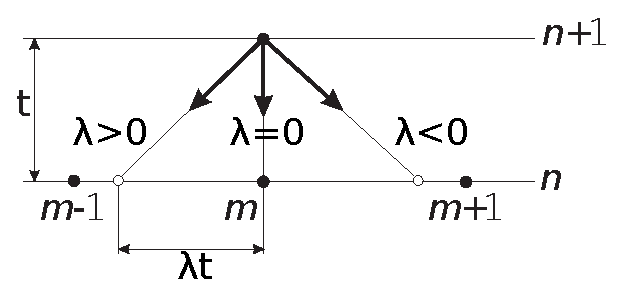
\includegraphics[width=0.5\textwidth]{eps/gcm-idea.eps}}
\caption{Принципиальная схема сеточно-характеристического метода.}
\end{figure}
Из точки пересечения характеристики со слоем $n$ значение $v_i$ переносится в 
точку $\xi^{n+1}_m$ путём решения \ref{advection_equation_final}:
$$v_i^{n+1}(\xi_m)=v^{n}_i(\xi_m-\lambda_i\tau) + {\tilde f}_i \tau.$$
Если характеристика не попадает точно в расcчётный узел, то применяются различные
методы реконструкции значения в данной точке (в данной работе используется
интерполяция соответствующего порядка).
\subsubsection{Расщепление по пространственным направлениям}				
Идея метода \cite{fedorenko} решения исходной задачи состоит в расщеплении по трём пространственным координатам, то есть в разделении на этапе численного решения трёхмерной системы уравнений \ref{matrix_equation} на три одномерных. На уровне дифференциальных операторов это может быть записано следующим образом:
\begin{equation}
\frac{\partial}{\partial t}\vec u+\mathbf{A}_x \frac{\partial}{\partial x}\vec u
= \vec f,
\label{matrix_equation_x}
\end{equation}
\begin{equation}
\frac{\partial}{\partial t}\vec u+\mathbf{A}_y \frac{\partial}{\partial y}\vec u
= \vec f,
\label{matrix_equation_y}
\end{equation}
\begin{equation}
\frac{\partial}{\partial t}\vec u+\mathbf{A}_z \frac{\partial}{\partial z}\vec u
= \vec f,
\label{matrix_equation_z}
\end{equation}
Эти уравнения решаются последовательно описанным в предыдущем параграфе методом с использованием
на очередном подшаге результатов, полученных на предыдущем подшаге.

\subsubsection{Расчёт граничных узлов}
Описанный выше чистый метод характеристик применяется только для расчёта внутренних узлов
сетки, то есть в том случае, если выпущенная из точки характеристика не
выходит за пределы области интегрирования. В противном случае для нахождения значений на новом временном слое  составляется система уравнений, в которой данные выводящих характеристик заменяются граничными и контактными условиями. Рассматриваемая система уравнений в граничных узлах имеет не более трёх
\cite{chelnokov} выводящих характеристик. 

Граничные условия могут быть нескольких видов, например (символы без волны -- для первого тела, с волной -- для второго):
\begin{itemize}
\item{жёстко закреплённая граница
\begin{eqnarray}
v_\tau=v_n=0; \nonumber
\end{eqnarray}}
\item{свободная граница
\begin{eqnarray}
\sigma_\tau=\sigma_n=0; \nonumber
\end{eqnarray}}
\item{скольжение тел друг относительно друга 
\begin{eqnarray}
v_n=\tilde{v}_n,\nonumber\\
\sigma_n=\tilde{\sigma}_n,\nonumber\\
\sigma_\tau=\tilde{\sigma}_\tau=0; \nonumber
\end{eqnarray}}
\item{слипание тел
\begin{eqnarray}
v_n=\tilde{v}_n,\nonumber\\
v_\tau=\tilde{v}_\tau.
\end{eqnarray}}
\end{itemize}
Эти условия доопределяют СЛАУ на значения инвариантов Римана на новом временном слое.

\subsection{Пластический корректор}
В данной работе был реализован простейший корректор, реализующий нормировку вектора напряжений. Этот способ известен как правило корректировки Уилкинса\cite{wilkins}, и верен только для идеальнопластической среды без упрочнения.

Рассчитанные в ходе эластичного предиктора напряжения в случае выхода за поверхность текучести  $f(\sigma_{ij}) \geq 0$ (см. \ref{mizes}), возвращаются на неё путём умножения на нормировочный коэффициент:
\begin{eqnarray}
s_{ij}^{n+1} = s_{ij}^e\frac{k_F}{J_2^e}	\\
J_2 = \sqrt{\frac{1}{2}s_{ij}s_{ij}}
\end{eqnarray} 